\chapter{Narrow-Band Topology Optimization on a Sparsely Populated Grid} 
\label{Chapter:Elasticity}
In the context of designing efficient solver, topology optimization, as an application, creates very interesting challenges to the numerical solvers. It desires high resolution, for many interesting details only emerges in high resolution simulation. It generates sparse domain, as in many scenarios only a fraction($<5\%$) of domain is filled in the final solution. It also creates high contrast ($1:10^{-9}$) material distributions. 

In this chapter, I present a design of efficient linear elasticity solver that is tailored for high resolution and sparse domain. Regarding the high contrast material distribution, I will demonstrate how it impairs the multi-linear multigrid solver's convergence rate, which inspired a design of stencil-aware interpolation scheme that drastically improves convergence rate in those situations.
\section{Topology Optimization Overview}
\begin{wrapfigure}{R}{0.45\textwidth}
\centering
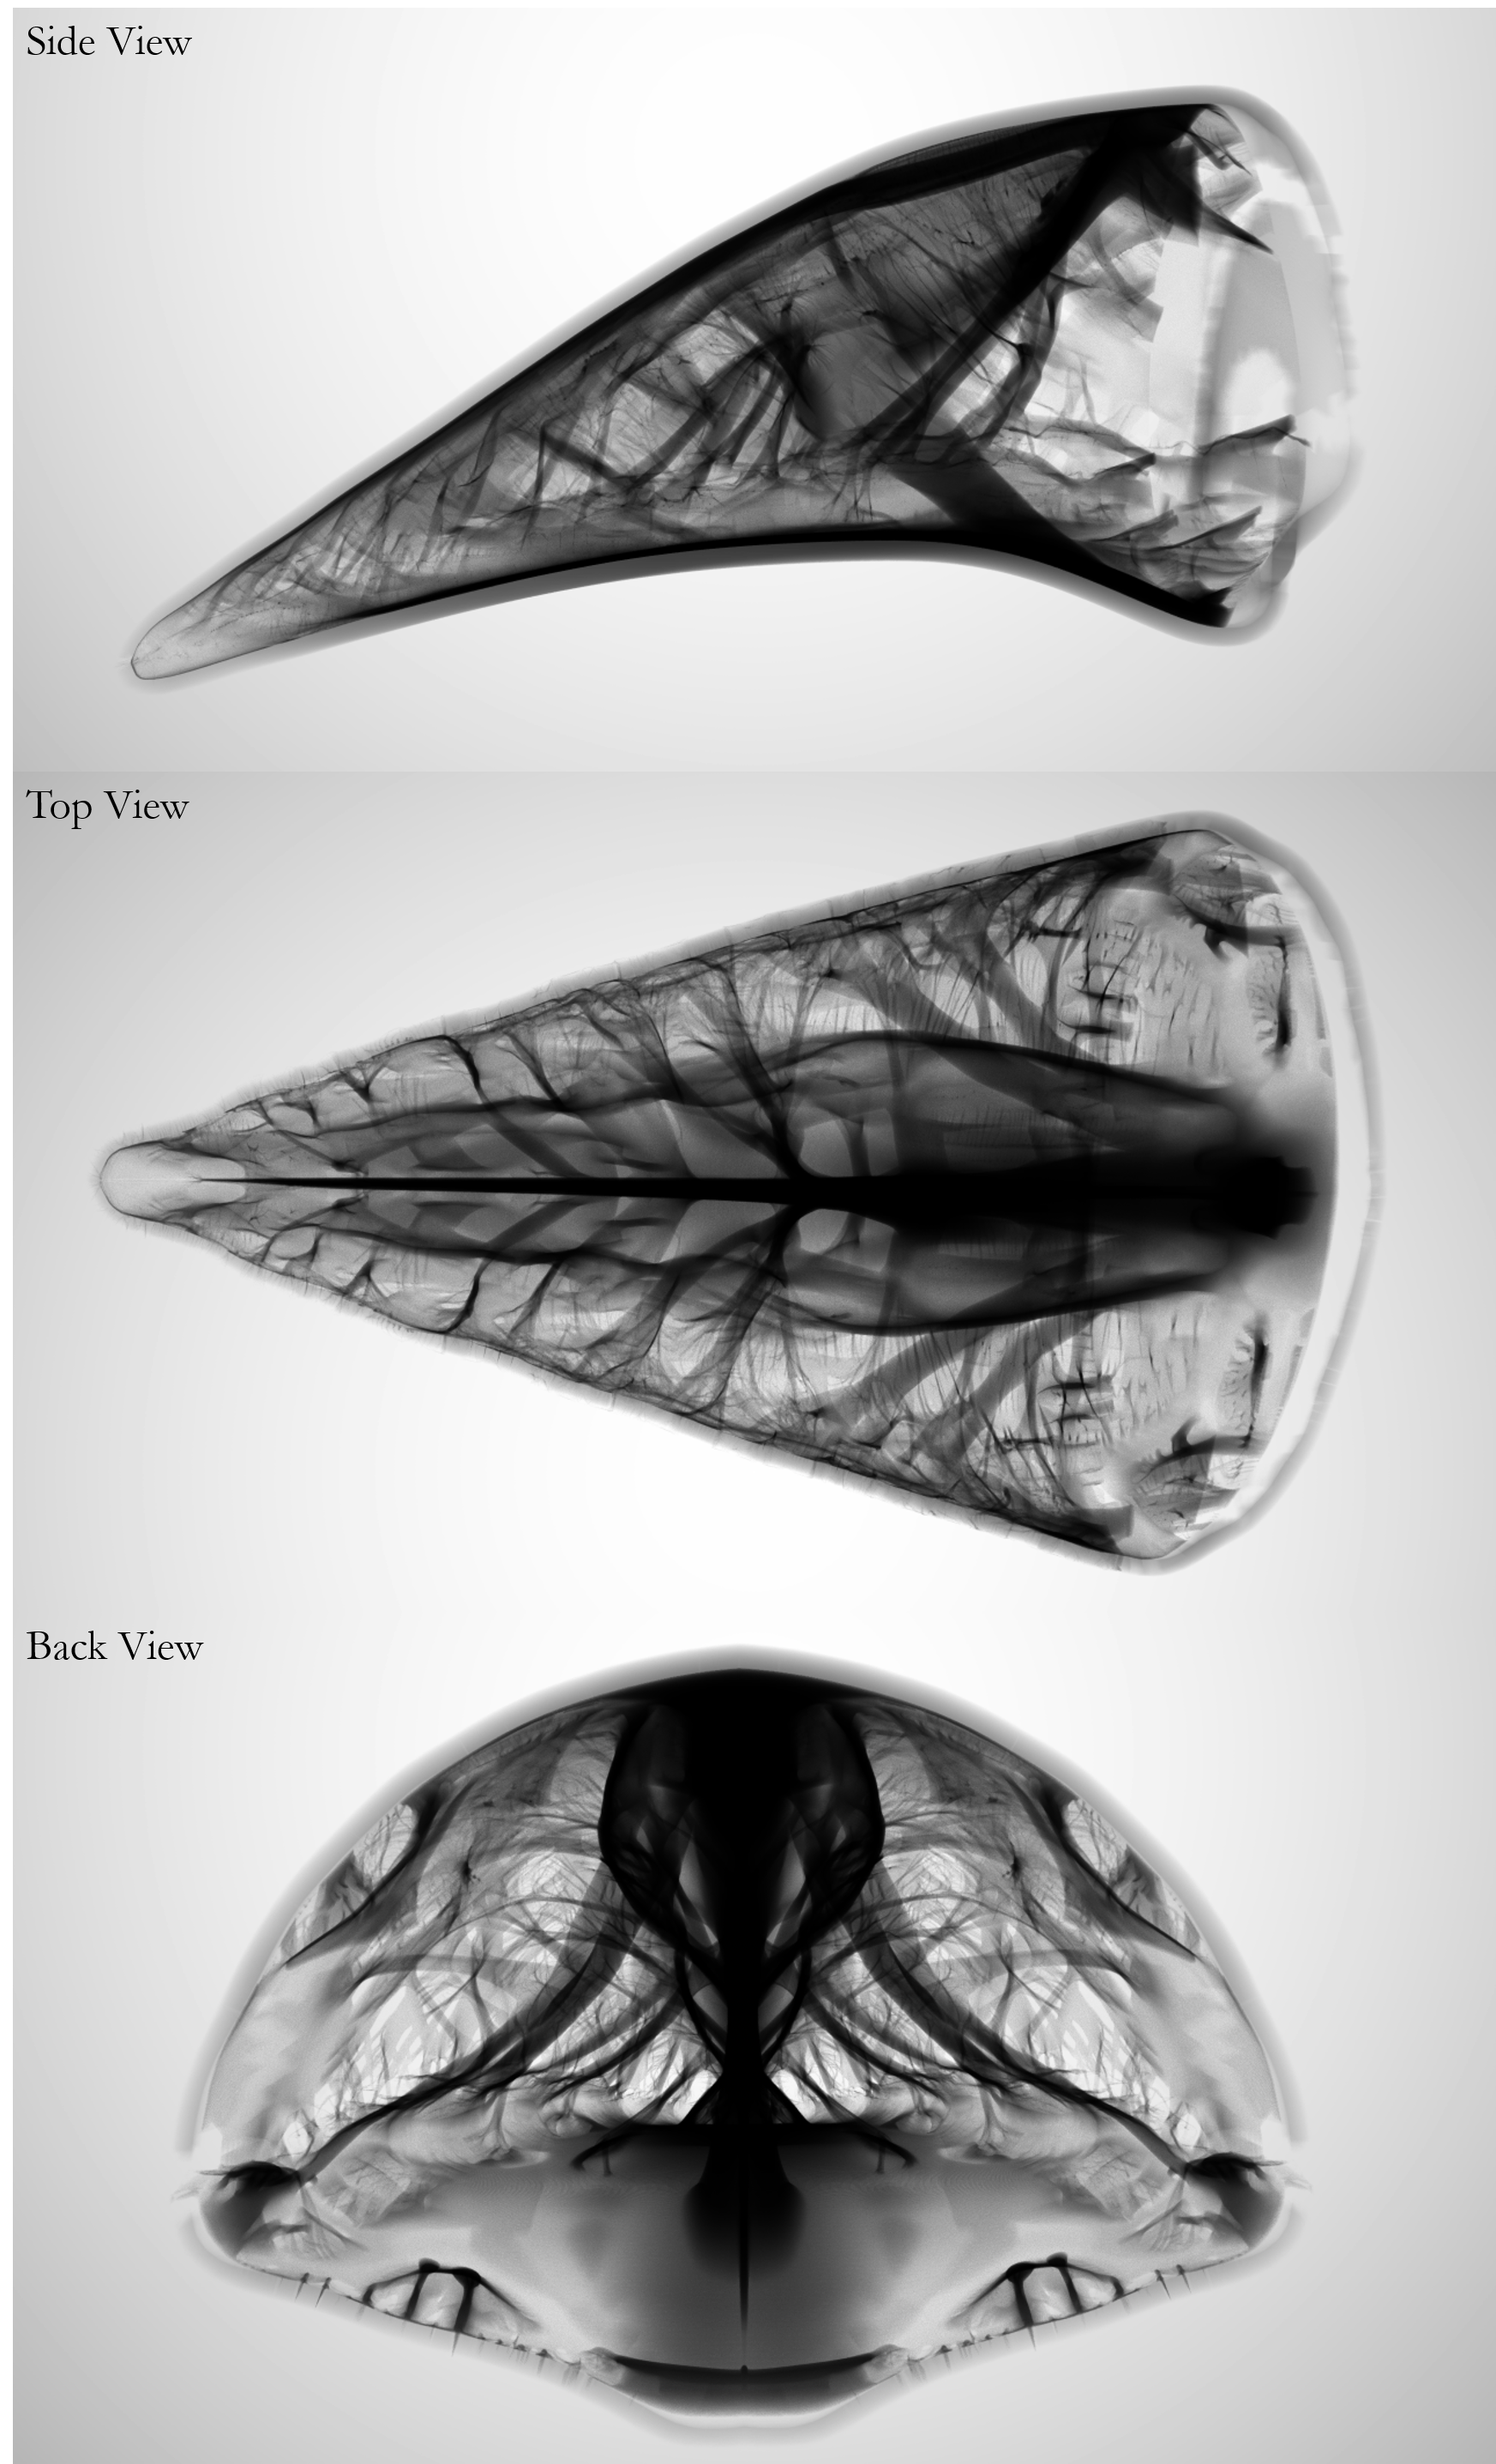
\includegraphics[width=0.42\textwidth]{images/TopOpt/beak_teaser}
\caption{The interior structures supporting the shell of a bird beak generated using our narrow-band topology optimization algorithm with $1,040,875,347$ (1.04 billion) active FEM voxels. The resolution of the background grid is $3000 \times 2400 \times 1600$. The three figures show the volumetric rendering of the same structure from different views.}
\label{fig:beak}
\end{wrapfigure}
Topology optimization aims to solve the problem of distributing materials in a given domain that minimizing the structural compliance or other objectives to given load(s).
It has demonstrated its efficacy in creating mechanical designs with complex structures and extreme properties in various engineering problems (see \cite{rozvany2009critical}, \cite{sigmund2013topology}, \cite{deaton2014survey} for surveys).
Starting from a volumetric domain that is uniformly filled with material, a standard topology optimization algorithm iteratively removes and redistributes material to develop a structure that minimizes a design objective (e.g., structural compliance), given the prescribed target volume and boundary conditions.  

However, due to the limitations of the previous computational frameworks, it is challenging to perform a standard topology optimization algorithm to emerge and evolve these thin and sparse features.
For example, to model the evolution of a thin sheet at the length scale of ten micrometers within a centimeter cube, it requires an FEM solver discretized on a $1000^3$ Cartesian grid. 
This grid resolution amounts to the order of magnitude of one billion active elements.

Recent advances in supercomputing provide some solutions that overcome this challenge.
For example, \cite{Aage2017GigavoxelCM} ran a parallel topology optimization program on a cluster with 8000 cores for days and obtained the structure of an airplane wing with the computational domain filled with 1.1 billion voxels.
A variety of novel, intricate, and multi-scale structures naturally emerge from the super-resolution computations.
This result is impressive, yet the limited accessibility and high cost of the supercomputing resources impede the use of such numerical approaches in a broader range of research and engineering applications. 
New computational tools, which are easy to access, efficient to run, and able to solve super-resolution systems, are needed in the scientific community.

\section{Main Contributions}
We propose a new computation framework that combines a sparse representation in conjunction with a highly optimized elastic multigrid solver for topology optimization, which delivers a significant leap in solving super-resolution problems from the prior state-of-the-art results.
Our framework has enabled the simulation of a sparsely populated computational domain on the level of billion active grid voxels on a single workstation. 
By examining the simulation results at such scale, we identify and analyze new challenges that have not been addressed, or even observed, in the previous research on elastic deformation simulation and topology optimization, such as poor asymptotic convergence of standard Galerkin-coarsened multigrid algorithm and the algorithmic limits of floating-point precision.

To address these scale-dependent challenges, we combined design practices and algorithmic interventions on data structures, numerical methods, and parallel solver implementations.
First, our framework is centered around a sparsely populated grid data structure, which allows the dynamic allocation of the degrees of freedom within a narrow band around the structure.  
This data structure combines the benefits of sparse storage, implicit topology representation, and the performance potential of high-throughput stream processing.
We have observed and demonstrated numerically that the elements with high structural sensitivities, which are essential for developing the structure towards its optimal topology, tend to bundle within a narrow band around the structure during evolution. 
In contrast, the vast bulk of void regions far from the structure contribute little to the total structural compliance, but they are the primary source of the computational cost in a dense discretization.
Therefore, the computation can be dramatically reduced by using a dynamically allocated sparse discretization, i.e the narrow-band representation.

In addition to the narrow-band representation, we developed a novel mixed-precision multigrid solver that is capable of solving FEM discretized linear elasticity in the order of billion elements on a single workstation.
By proposing an SPGrid-optimized matrix-free formulation for data storage and a novel mixed-precision computation, the solver can meet the memory storage and bandwidth demands of a multiprocessor workstation while maintaining high accuracy.
Also, our vectorized multigrid solver takes advantage of the AVX512 instruction set on the Intel Skylake-X/SP architecture in order to further enhance performance.

We summarize the main contributions of our work as follows:
\begin{itemize}
\item We demonstrate an ensemble of data structures, numerical schemes, and implementation best practices to perform topology optimization with the highest resolution (over one billion voxels) on a single shared-memory multiprocessor.
\item We propose a sparse, adaptive topology optimization framework where simulation of elastic deformation is restricted to a narrow band surrounding the high-density region.
\item We demonstrate the capacity of our framework to obtain a variety of complex thin and codimensional features, such as thin films and beams, that previous approaches might suppress.
\end{itemize}
\section{Method Overview}
Our sparse topology optimization framework consists of three key components: a sparse grid structure, a high-resolution multigrid FEM solver, and a narrow-band and unbounded structure optimizer. 
First, we briefly introduce the sparse paged structure (SPGrid) \cite{setaluri2014spgrid} as the base data structure to track the optimizing structures (Section \ref{sec:topopt_spgrid}). 
Next, we discuss our multigrid FEM solver for computing large-scale elastic systems on SPGrid in Section \ref{sec:topopt_multigrid}. 
Finally, in Section \ref{sec:topopt_result}, we provide method validations with respect to both the multigrid solver.

\section{Sparsely Populated Grid Structure}\label{sec:topopt_spgrid}
The Sparsely Populated Grid (SPGrid) data structure \cite{setaluri2014spgrid}, in comparison to other sparse  data structures, leverages the virtual memory system to allocate a very large virtual memory address span, corresponding to a sparsely populated background grid, while only materializing in physical memory the parts of this grid that are active. The allocation unit in SPGrid is a \emph{block}, a rectangular region of the Cartesian grid that is made contiguous in memory address space by virtue of a space-filling traversal scheme; The size of SPGrid blocks is chosen to be a multiple of a 4KB, i.e. the size of a physical memory page. SPGrid stores a number of data channels, which have similar sparsity pattern and corresponding indexing, in the same allocation block. Using the SPGrid data structure enables us to compute effectively on a sparsely populated domain with effective bandwidth comparable to a cache-optimized, dense uniform grid. In our multigrid FEM solver, we utilized the flexibility of SPGrid's block size, and chose a block size of $4\times 4\times 8$, tailored for vectorization as described in Section \ref{sec:topopt_multigrid}.
\section{Multigrid Solver}\label{sec:topopt_multigrid}
Our topology optimization framework utilizes a numerical solver for a lattice-based Finite Element Method (FEM) discretization of linear elasticity, with spatially varying material
parameters. In order to accommodate the large resolutions targeted by our method, we employ a solver based on the Multigrid-Preconditioned Conjugate Gradients (MGPCG)
algorithm. Algebraically, our methodology is similar to prior formulations of multigrid-preconditioned solvers [\cite{wu2016,dick2011real}], in employing a hexahedral discretization of
the linear elasticity operator, leveraging Galerkin coarsening to generate coarse level operators, and using a symmetric V-cycle as a preconditioner for Conjugate Gradients.
We deviate from standard practices as documented in prior work by way of design choices, data structures, and parallelization practices including: 
\begin{itemize}
\item A matrix-free implementation of the finest-level elasticity operator tailored for the SPGrid sparse storage structure.
\item A bandwidth-saving construction of the Galerkin coarsened operator at each level, which avoids streaming through explicitly-built matrices as input any only relies on
material properties at the finest level.
\item Storage of the explicitly formed coarse grid operators in a novel, SPGrid-specific banded sparse matrix format.
\item A modified eight-color Gauss-Seidel smoother designed to optimize memory bandwidth utilization and SIMD efficiency.
\item A mixed-precision implementation of MGPCG, which combines the accuracy of double-precision arithmetic with the storage saving
of single-precision representations.
\end{itemize}

\paragraph{Matrix-free design of finest level operator.} Due to the size of the simulation domains we target, economy in
memory footprint is essential to our approach. An explicit matrix storage at any level of the discretization would
necessitate 243 scalar coefficients per lattice node, consisting of 27 spokes of $3\times 3$ matrices. This number excludes
any compaction afforded by storing only the symmetric half of the operator, but also does not account for any additional
storage of matrix indices (e.g. in compressed sparse row format), or explicit topology storage of the computational
domain (e.g.  explicit hexahedral mesh). 

The SPGrid data structure provides the abstraction of a sparsely populated grid, without the need to explicitly
encode the connectivity of hexahedral simulation elements (e.g. as in an explicit mesh structure), as it is implied by
the background uniform grid topology. Although our computational domain is embedded in a large background regular grid
(up to the resolution of $3000\times 2400\times 1600$), its active cells in our simulation are only a sparse subset (up to 1.04 billion active cells, in our tests). The SPGrid structure allows us to directly store these active cells,
their material parameters as well as their nodal forces and displacements in a
sparsely populated grid. 

At the finest level, we
implemented a numerical kernel that computes the elastic forces resulting from the elasticity operator, for all nodes of a
given $4\times 4\times 8$ block of the SPGrid structure; this kernel is designed to be free of write-dependencies, hence
all blocks can be processed in parallel on different threads.

Consider a single grid cell with nodal displacements $\{\mathbf{u}_i\}_{i=1}^8$. We denote by $\{\mathbf{f}_i\}_{i=1}^8$
the nodal forces produced by the elastic response of the same cell, which can be expressed as 
$\mathbf{f}_i = \sum^8_{j = 1} \mathbf{K}_{ij} \cdot \mathbf{u}_j$. Each $\mathbf{K}_{ij}$ in this expression is a
$3\times 3$ matrix; we store these coefficients in a $8\times 8\times 3\times 3$ tensor $\mathcal{K}$, whose elements
are given by $\mathcal{K}_{ijvw}=[\mathbf{K}_{ij}]_{vw}$. This tensor is given as a linear combination of two canonical
tensors $\mathcal{K}^\mu$ and $\mathcal{K}^\lambda$\changed{}{ based on the Lam\'{e} coefficients}, corresponding to the stiffness matrices computed for
$(\mu,\lambda)=(1,0)$ and $(\mu,\lambda)=(0,1)$ respectively. \changed{It should be noted that $\mathcal{K}^\mu$ and
$\mathcal{K}^\lambda$ can either be computed by analytic integration of the linear elastic potential trilinear element}{They can be computed either by analytic integration of the linear elastic trilinear element},
or an eight-point Gauss quadrature rule. Ultimately, the elemental stiffness
tensor is expressed as $\mathcal{K}=\mu\mathcal{K}^\mu+\lambda\mathcal{K}^\lambda$. 
We use the notation $\mathcal{C}(i)$ for the set of eight cells incident to node $i$, while $\mathcal{V}(c)$ denotes the eight vertices at the corners of cell $c$. We can then express the total force on node $i$ as:
$$
\mathbf{f}_i = \sum_{c \in \mathcal{C}(i)} \sum_{j\in \mathcal{V}(c)} (\mu^{(c)} \cdot \mathbf{K}^\mu + \lambda^{(c)} \cdot \mathbf{K}^\lambda)_{i^{(c)}j^{(c)}} \cdot \mathbf{u}_j
$$
where $\mu^{(c)},\lambda^{(c)}$ are the parameters of cell $c$, and $1\leq i^{(c)},j^{(c)}\leq 8$ are the local indices of nodes $i,j$ as vertices of cell $c$. 
This operation can be trivially vectorized; let $\underline{\mathbf{f}}:=(f_{(p,q,r)},f_{(p,q,r+1)},\ldots,f_{(p,q,r+7)})$ be a SIMD vector of eight forces on nodes that are sequential along the $z$-axis, while $\underline{\mu}^{(c)}, \underline{\lambda}^{(c)}$ are the parameters of a cell neighbor for each of the eight sequential grid indices, and finally, $\underline{\mathbf{u}}_j$ the set of eight sequential nodal neighbors at a specific offset direction. The previous operation is then expressed as:
\begin{equation}
\underline{\mathbf{f}} = \sum_{c \in \mathcal{C}(i)} \sum_{j\in \mathcal{V}(c)} (\underline{\mu}^{(c)} \cdot \mathbf{K}^\mu + \underline{\lambda}^{(c)} \cdot \mathbf{K}^\lambda)_{i^{(c)}j^{(c)}} \cdot \underline{\mathbf{u}}_j .
\label{eqn:elasticity-stencil}
\end{equation}
We note that a SIMD line need not be structured strictly along a sequence of nodes aligned along the $z$-axis (or any other single axis); a rectangular arrangement, e.g. eight nodes straddling a $2\times 4$ rectangle along the $y$- and $z$-axes would work in exactly the same fashion. From a programming standpoint, equation (\ref{eqn:elasticity-stencil}) indicates that SIMD vectors of each Lam\'{e} parameter are scaled with a constant coefficient (a single multiply instruction, with embedded broadcast, in the AVX2 and AVX512 instruction sets), and multiply the respective neighboring displacements $\underline{\mathbf{u}}_j$ (a fused multiply-add operation) to compute a term contributing to
the nodal force $\underline{\mathbf{f}}$. With the increased number (32) of available registers in AVX512, we have verified that the entire stencil application can be executed with $2\times
24^2$ multiply and $2\times 24^2$ fused multiply-add instructions (FMA) without any register spilling, and enough distance between operation dependencies to allow the full throughput of \changed{2}{two}
FMA instructions per cycle in Skylake-X/SP\footnote{Intel Xeon Gold 6140 processor (18 cores at 2.30 GHz) with $192$ GB memory.} (approximately 1200 cycles for the stencil application on one 16-wide SIMD line).

\paragraph{Modifications to the SPGrid structure} In order to accommodate the SIMD-heavy stencil computations in our elasticity operator, we enacted two crucial modifications/enhancements of the baseline implementation \textsf{(http://www.cs.wisc.edu/\char`~sifakis/SPGrid.html)} of the SPGrid structure of \cite{setaluri2014spgrid}. The first of those, is a vectorized load routine, with a compile-time stencil offset, as in:
\begin{shaded}
\texttt{template <int di,int dj,int dk,class SPG\char`_array>}\\
\texttt{\char`_\char`_m512 VectorGet<di,dj,dk>(SPG\char`_Array a,int64\char`_t offset)}
\end{shaded}
where a 16-entry SIMD width in single-precision has been used, as an AVX512 example. The offset given as argument is presumed aligned at SIMD-width granularity, while a stencil offset 
$\texttt{(di,dj,dk)}$ is given as a compile-time argument. Using these semantics, grid data at a given stencil ``spoke'' (from an aligned baseline vector address) can be loaded for an entire SIMD line, as illustrated in Figure\ref{fig:simd_get}.
\begin{figure}[h] 
\center
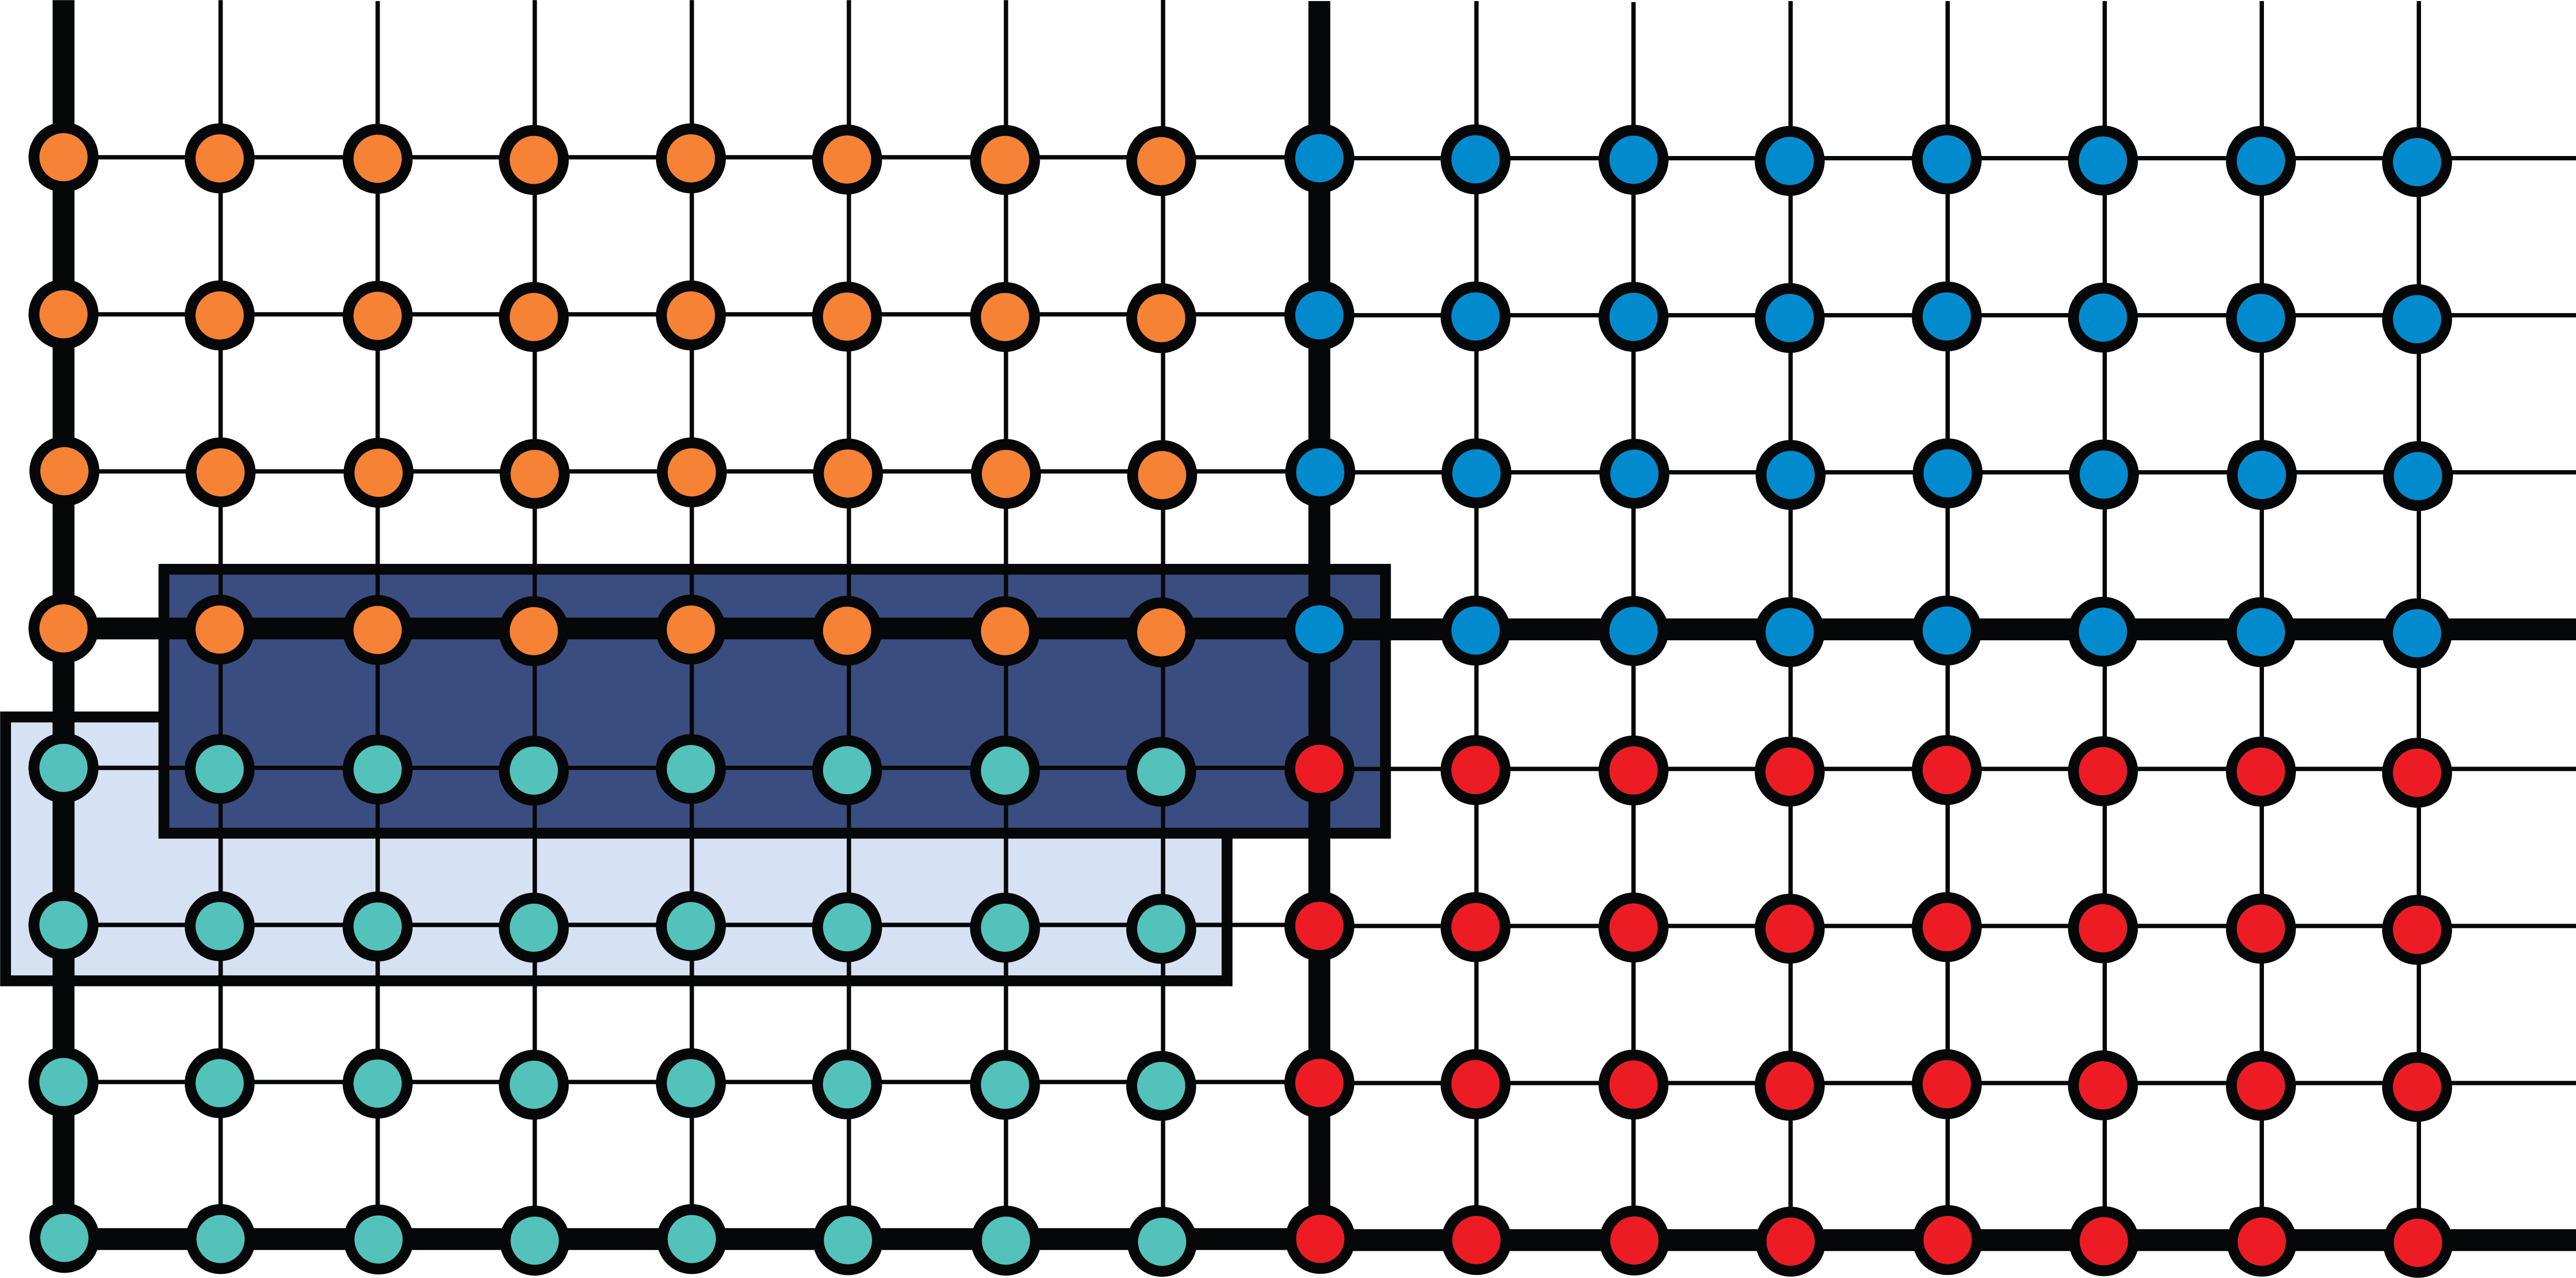
\includegraphics[width=.5\textwidth]{images/TopOpt/SIMD_Get}
\caption{The $\texttt{offset}$ passed to $\texttt{VectorGet}$ points to an sequence of SPGrid entries with SIMD-width alignment (light blue box). Using a stencil offset, e.g., shifts the region to be loaded by $\texttt{VectorGet}$, as shown in the dark blue box. The data of this shifted box may originate in several distinct SPGrid blocks (indicated by different node colors).}
\label{fig:simd_get}
\end{figure}
\noindent Even though the stencil shift might cause data to originate from different SPGrid blocks, the fact that such shift is known at compile time allows significant optimizations that avoid expensive gather operations and minimize address translations. 

The second SPGrid modification was the relaxation of the design restriction in \cite{setaluri2014spgrid} that each SPGrid block be sized to exactly 4KB (the size of a virtual memory page). Our solver used a total of $128$ bytes for all variables stored at each grid index, leaving the block size to just $2\times 4\times 4$ when a 4KB block size is used. We found it more effective to be able to use a larger block size, namely $4\times 4\times 8$ in order to (a) minimize the number of SIMD stencil accesses that straddle multiple blocks, and simplify implementation of $\texttt{VectorGet}$, and (b) allow an adequate number of nodes to be present per-block, to ensure that even after eight-coloring (as required by our smoother, described later in this section), the nodes on each color are a multiple of the SIMD width, even on AVX512 systems. We include source code for both proposed SPGrid modifications, as a supplement to our paper. As an indication of performance, we have achieved an effective bandwidth of $17.45$ GB/s for our multiply kernel.


\paragraph{Efficient Galerkin Coarsening.} In the construction of the multigrid hierarchy, we used the Galerkin coarsening method, computing the coarse grid operator as 
$\mathbf{K}^{c} = \mathbf{P}^T \cdot \mathbf{K}^{f} \cdot \mathbf{P}$, where $\mathbf{P}$ is the prolongation matrix and $\mathbf{K}^{f}$ the fine grid operator. At all but the two finest
levels, we can afford to store the coarsened operator explicitly, as the reduced dimensionality of the coarse grid allows us to do so at one-eighth of the memory footprint that such
matrix would have occupied at the finer level. Our construction of $\mathbf{K}^{c}$ is tailored around the following implementation objectives:
\begin{itemize}
\item Neither $\mathbf{K}^{f}$ or $\mathbf{P}$ are presumed available in matrix form.
\item The rows of $\mathbf{K}^{c}$ should be computed independently, to avoid write hazards.
$^\dagger$\item We seek the flexibility to compute $\mathbf{K}^{c}$ at \emph{any} coarse level directly from the material parameters at the finest level, without depending on operators
  at intermediate levels.
\end{itemize}

\begin{wrapfigure}{r}{.35\textwidth}
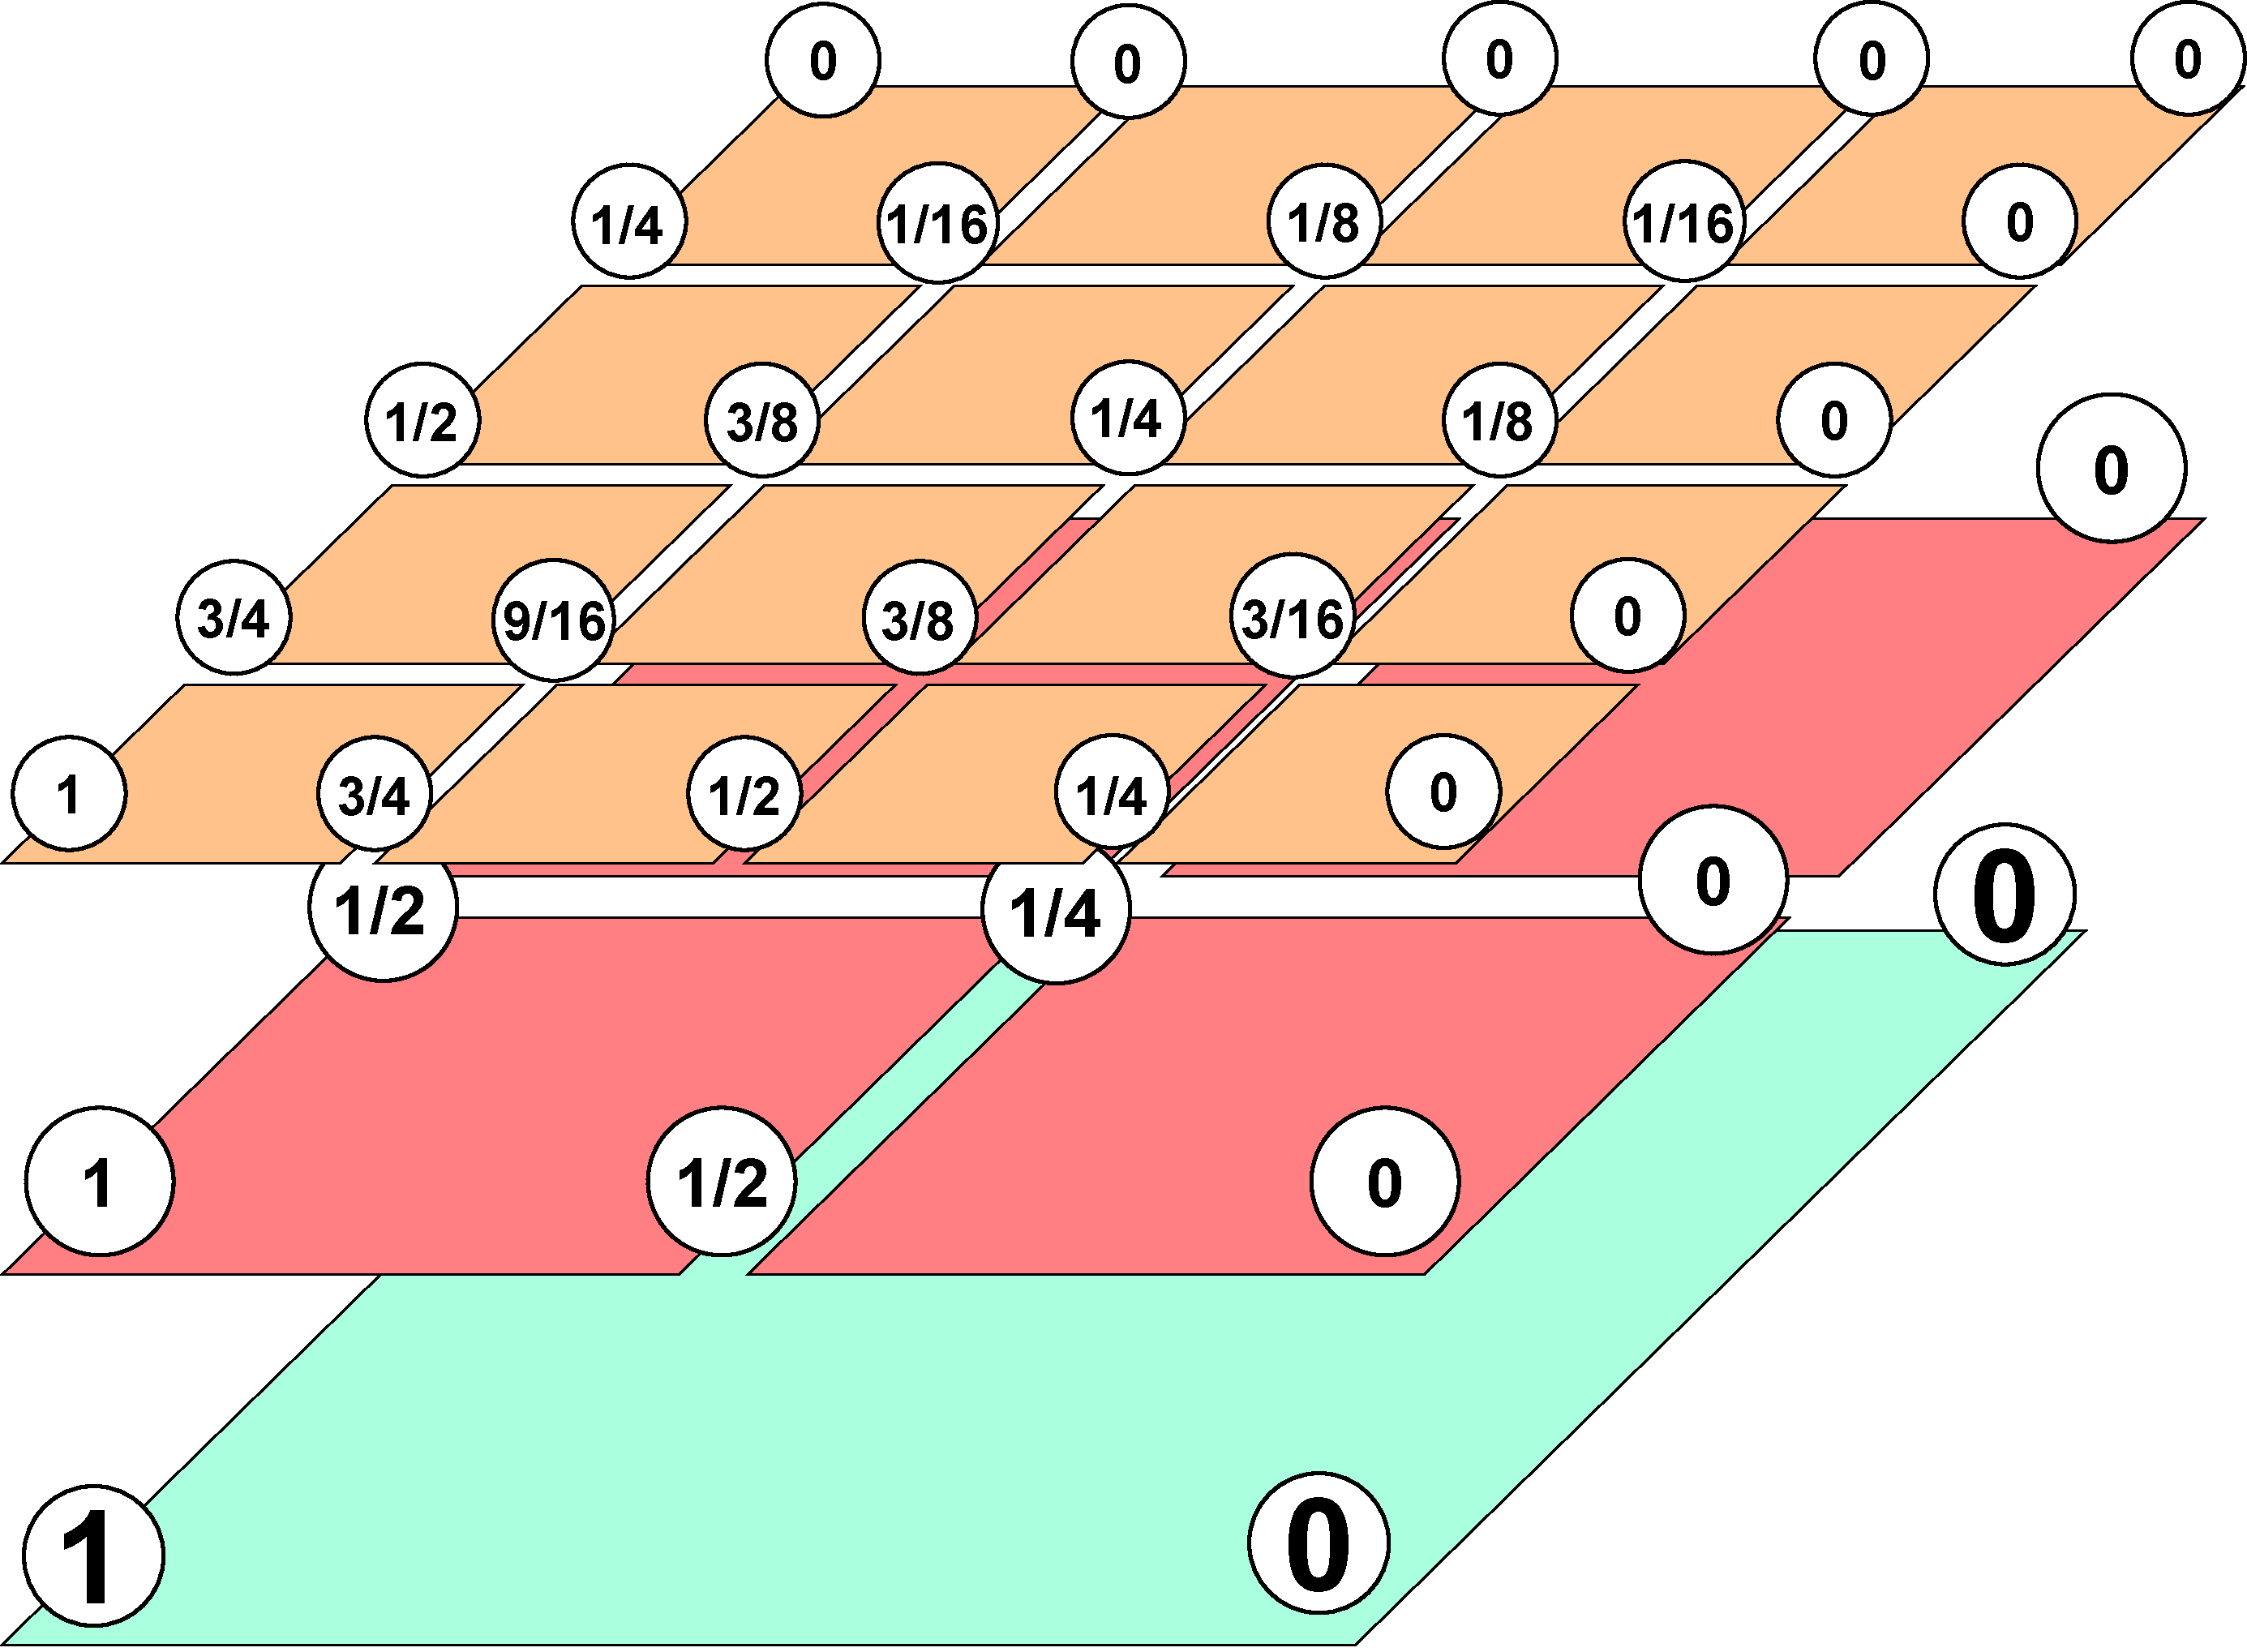
\includegraphics[width=.3\textwidth]{images/TopOpt/prolongation_v2}
\caption{Two successive prolongation operations on a Kronecker delta function during Galerkin coarsening of a coarse cell, illustrated in 2D.}
\label{fig:prolongation}
\end{wrapfigure}

Let us consider the specific example of constructing the operator $\mathbf{K}^{4h}$ at two levels coarser from the finest grid:
\begin{equation}
\mathbf{K}^{4h}=\mathbf{P}_{4h\rightarrow 2h}^{T}\mathbf{P}_{2h\rightarrow h}^{T}\mathbf{K}^h\mathbf{P}_{2h\rightarrow h}\mathbf{P}_{4h\rightarrow 2h}
\label{eqn:galerkin}
\end{equation}
The coefficients of the $i$-th row of this matrix (or equivalently, the $i$-th column, due to symmetry) are given by the action $\mathbf{K}^{4h}\mathbf{e}_i$ of this operator on the
basis vector $\mathbf{e}_i$. Equation (\ref{eqn:galerkin}) suggests that this action can be computed by successively prolongating $\mathbf{e}_i$ to the finest level, applying the
fine-grid operator $\mathbf{K}^{h}$, and restricting the result back to the coarse grid. 
We perform this operation separately on each of the eight cells (at level $4h$) incident on node $i$,
as illustrated in Figure~\ref{fig:prolongation}. The input to this process is a discrete Kronecker delta, shown as the input coefficients to the coarsest level. 
We can use an eight-wide SIMD register to store all eight nodal values of this
coarse cell. We have implemented a routine $\textsf{ProlongateCell()}$ that interpolates this eight-value SIMD register into eight more eight-wide registers corresponding to the nodal values of
the child cells at the immediate finer level. This routine is called recursively to prolongate all the way to the finest level. At that point, a routine $\textsf{CellMultiply()}$ is used
to compute the force response of each individual fine cell to these prolongated nodal displacements (using the material properties at the finest level). 
A routine $\textsf{RestrictCell()}$ implements the adjoint of the prolongation operation by collecting force contributions from fine child cells to their coarser parent. Since these routines are
called recursively, all SIMD vectors are stack-allocated and can be effectively cached.
As an indicator of performance, the construction of the entire operator hierarchy in our 1.04\changed{B}{ billion-}voxel example (Figure \ref{fig:beak}) requires 113.9 seconds using AVX512 instructions, which is a very small fraction of the MGPCG cost at this resolution.


\paragraph{Sparse Matrix Storage} The storage of the Galerkin-coarsened matrix needs to be handled as to exploit sparsity, facilitate the application of the smoother routine,
and allow a direct solver (in our case, Intel MKL PARDISO) to be used for solving the problem at the coarsest level of the hierarchy. Given that the topology of the background is a regular
Cartesian lattice, we use a band-storage approach, where the 243 nonzero coefficients associated with the stencil each node (a $3\times 3$ matrix for every spoke of a 27-connected
$3\times 3\times 3$ stencil) are stored into a secondary SPGrid structure. We supplement these 243 scalars with a bit field,
indicating whether each stencil spoke is structurally present in our discretization. This representation allows straightforward implementation of the smoother routine, and can be easily
converted to compressed sparse row (CSR) format for usage in direct solvers like PARDISO. In this conversion, the only serial operation is the calculation of linearized indices, and the necessary
allocated length of each compressed row; the data transfer into the CSR coefficient buffer is performed in parallel over SPGrid blocks.

\paragraph{Optimization of the relaxation routine} In order to balance convergence efficiency with parallelization potential, we employ an eight-color Gauss-Seidel (GS) routine, as other
authors have similarly adopted in prior work \cite{wu2016}, with the slight modification that we collectively update all three collocated degrees of freedom at each grid node, by inverting
the $3\times 3$ diagonal block of the stiffness matrix corresponding to that node. A drawback of combining the eight-color GS smoother with a SIMD implementation is the suboptimal
utilization of memory bandwidth, as each SIMD vector will require data that is consistently discontinuous in memory (Figure \ref{fig:gs_blocks}, left). Such scattered memory assess is
particularly wasteful for modern hardware which always performs load operation from memory at cache-line granularity. In order to circumvent the need for such scattered data access, we
preemptively transpose the data in each SPGrid block as to reorder the indices of each color to be consecutive in memory (Figure \ref{fig:gs_blocks}, right/bottom). We observe that applying the
same stencil offset to the nodes of one color always leads to nodes of a different yet consistent color (e.g., in Figure \ref{fig:gs_blocks}, applying a (+1,+1) offset to a yellow node
always leads to a red node). As a consequence, after the described transposition, applying the colored GS smoother on each individual color can be performed by a straightforward
application of the $\texttt{VectorGet}$ routine to the transposed data. Each SPGrid block is transposed back to the original ordering at the end of the application of the
relaxation routine. We have observed an effective bandwidth of up to $68$ GB/s (out of maximum $128$ GB/s) on a Skylake-SP platform for the eight-color GS routine.


\begin{figure}[t] 
\begin{subfigure}[b]{.5\textwidth}
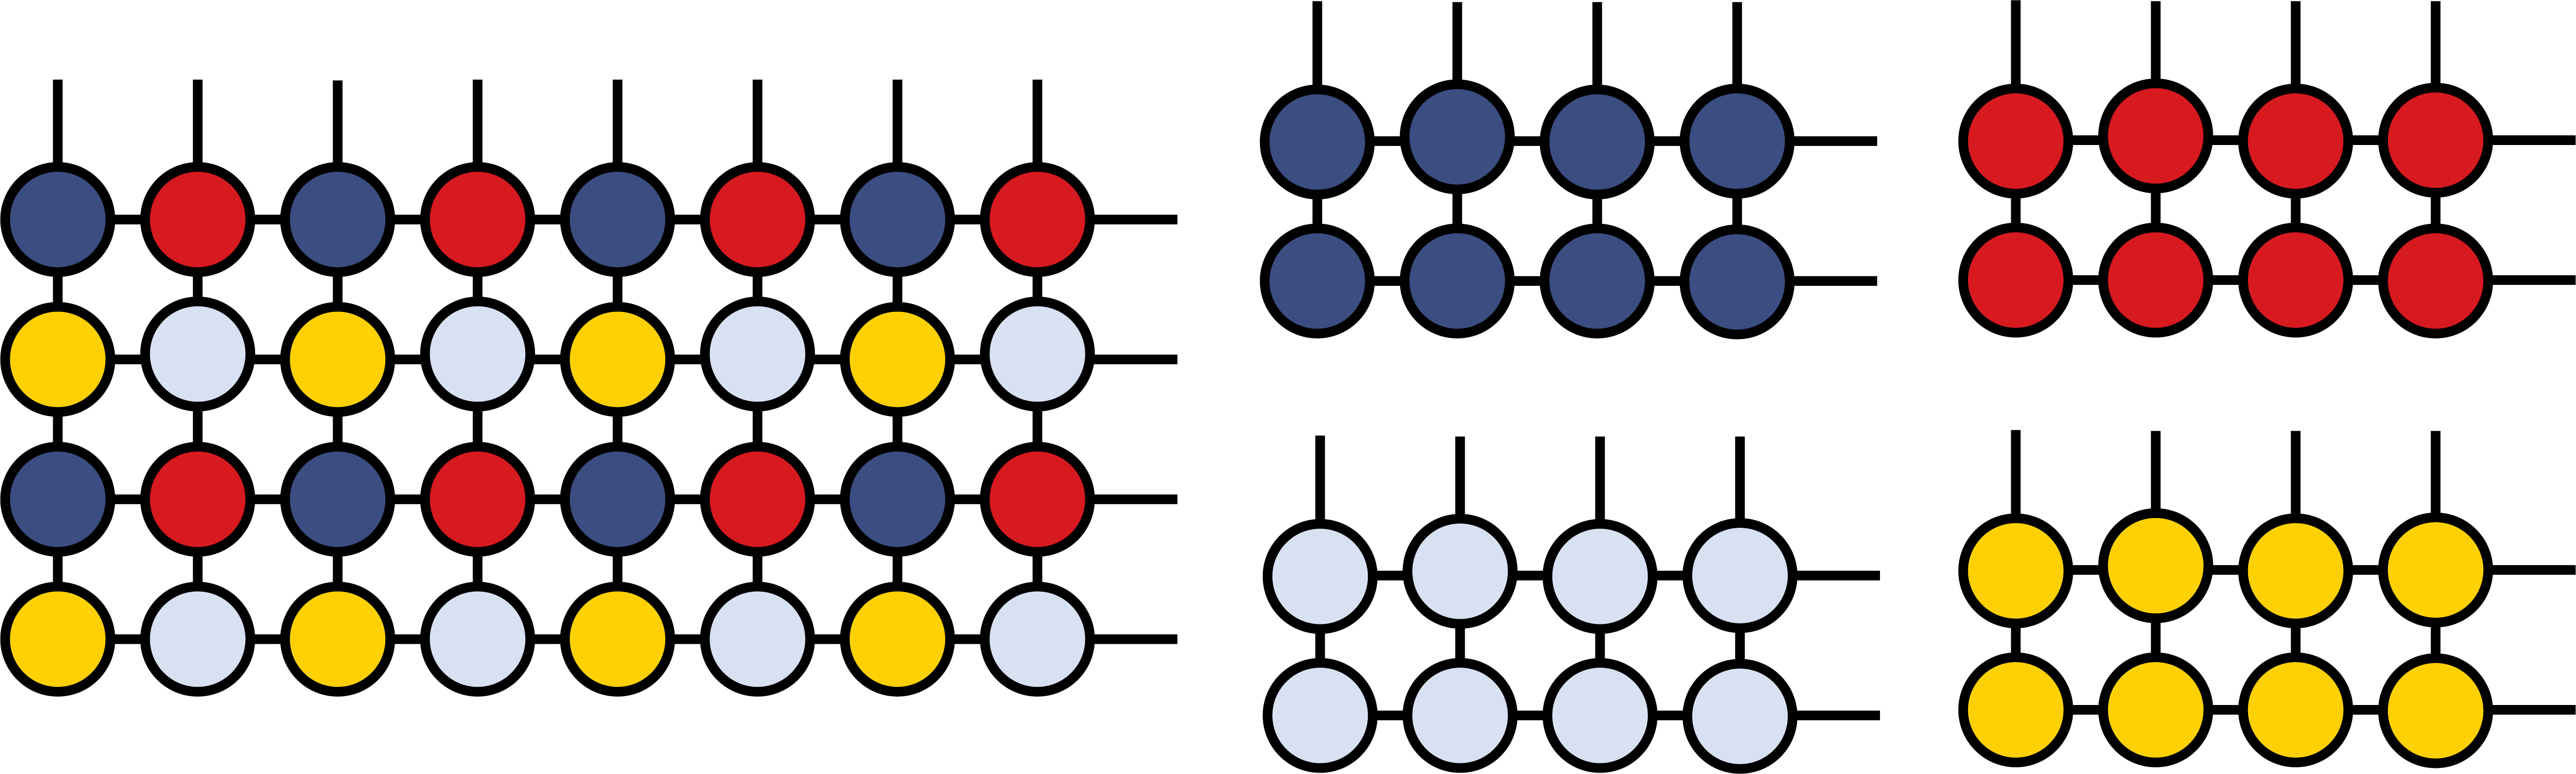
\includegraphics[width=0.9\textwidth]{images/TopOpt/GS_Grid}\\
\end{subfigure}
\begin{subfigure}[b]{.5\textwidth}
\raisebox{0.8cm}{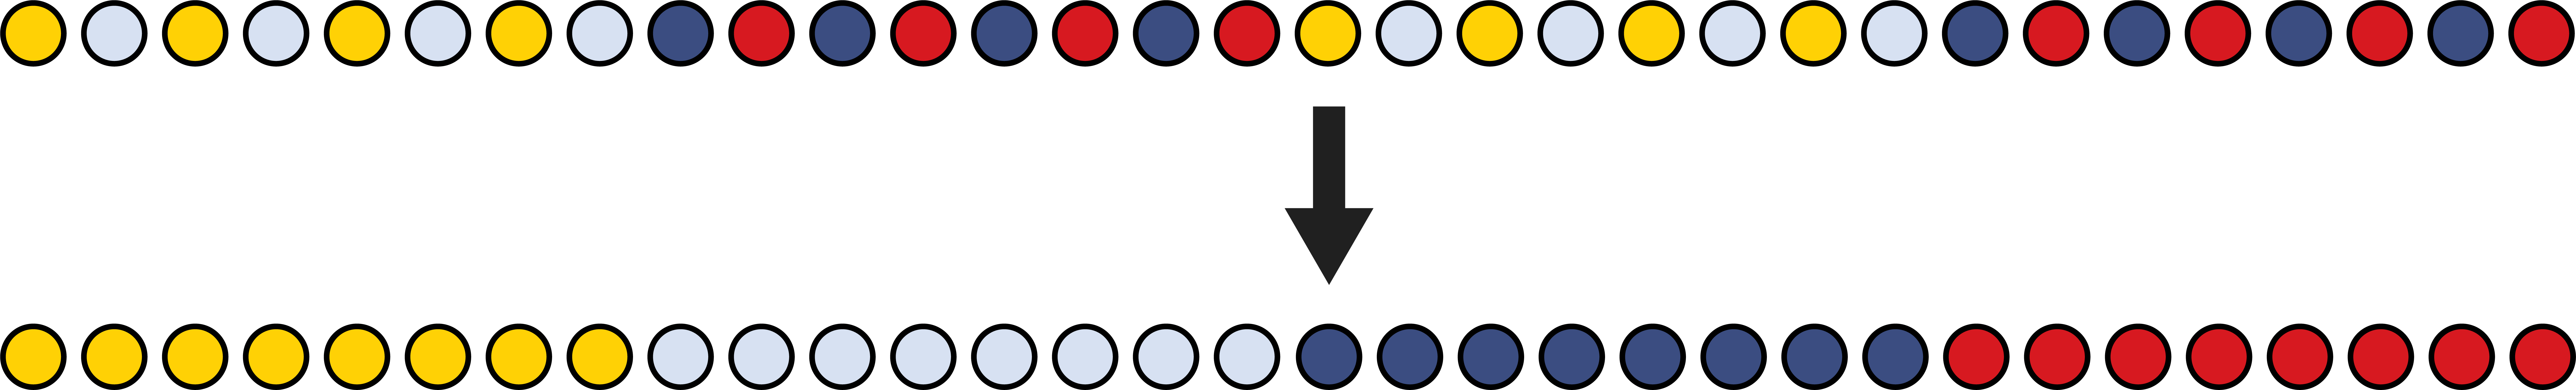
\includegraphics[width=0.9\textwidth]{images/TopOpt/GS_Grid_Linear}}
\end{subfigure}
\caption{Left: a SPGrid block of 4x8 in which the nodes are ordered lexicographically, Right: the transposed colored storage enables efficient vectorization for Gauss-Seidel iteration.
Bottom: Transposition operation of a SPGrid block illustrated in a linear memory layout.}
\label{fig:gs_blocks}
\end{figure}

\paragraph{A mixed-precision MGPCG solver} The linear systems arising from the equations of elasticity in our large-scale topology optimization tasks impose a unique set of
challenges to the numerical algorithms used. Due to both the sheer size of the computational domains we seek to accommodate, and the large contrast of material stiffness values used in
different regions of the simulated domain, we often encounter situations where an MGPCG solver using single-precision (32-bit) floating-point arithmetic cannot sustain satisfactory
convergence, or even instances where the solver will plainly diverge. There are also scenarios where single precision will have catastrophic consequences on our solver, when
Galerkin-coarsened matrices will be reported as effectively ``singular'' by direct solvers (i.e. MKL PARDISO) if constructed to single precision. We note that the frequency of incidence
of such issues was dramatically increased, in our experience, when dealing with domains in excess of $10^8$ voxels, while lower-resolution problems would be significantly more resilient.

An MGPCG solver implemented natively in double precision was fully effective for all the examples in our paper. However, using double precision would double our memory footprint, which
was a significant concession given our pursuit of exceptionally high-resolution domains. We thus designed a variant of such solver that used a carefully crafted mix of single- and
double-precision arithmetic, which we have found to produce results of effectively identical accuracy as a native double-precision solver. Consider the main loop of a 
preconditioned conjugate gradients algorithm, as captured in the following pseudocode:
\begin{figure}[h]
\center
\fbox{
\begin{minipage}{5.5cm}
\vspace*{-.2in}
\begin{align}
\mbox{\textbf{for}}\ \ k=1:N\hspace*{-.3in}\nonumber\\
\color{blue}{\mathbf{q}_k} &\leftarrow \color{purple}{\mathbf{A}}\color{blue}{\mathbf{p}_k}\label{eqn:op-multiply} \\
\color{blue}{\alpha_k} &\leftarrow \color{blue}{\mathbf{r}_k}^{\color{black}{T}} \color{blue}{\mathbf{z}_k} \color{black} / \color{blue}{\mathbf{p}_k}^{\color{black}{T}} \color{blue}{\mathbf{q}_k}\nonumber \\
\color{purple}{\mathbf{x}_{k+1}} &\leftarrow \color{purple}{\mathbf{x}_{k}} \color{black}{+} \color{blue}{\alpha_k} \color{blue}{\mathbf{p}_k}\label{eqn:x-acc}\\
\color{blue}{\mathbf{r}_{k+1}} &\leftarrow \color{blue}{\mathbf{r}_{k}} \color{black}{-} \color{blue}{\alpha_k} \color{blue}{\mathbf{q}_k}\nonumber\\
\color{blue}{\mathbf{z}_k} &\leftarrow \color{purple}{\mathbf{M}^{-1}}\color{blue}{\mathbf{r}_k} \label{eqn:preconditioner}\\
\color{blue}{\beta_k} &\leftarrow \color{blue}{\mathbf{z}_{k+1}}^{\color{black}{T}}\color{blue}{\mathbf{r}_{k+1}} \color{black} / \color{blue}{\mathbf{z}_{k}}^{\color{black}{T}}\color{blue}{\mathbf{r}_{k}} \nonumber\\
\color{blue}{\mathbf{p}_{k+1}} &\leftarrow \color{blue}{\mathbf{z}_{k+1}} \color{black}{+} \color{blue}{\beta_k} \color{blue}{\mathbf{p}_k}\nonumber
\end{align}
\end{minipage}
}
\end{figure}
Our modifications which yield a mixed-precision implementation are summarized as follows:
\begin{itemize}
\item Vectors $\mathbf{r},\mathbf{q},\mathbf{z}$ and $\mathbf{p}$ (colored blue, above) are persistently stored in single-precision floating-point variables. 
\item The solution $\mathbf{x}$ is stored in double precision. The accumulation operation in (\ref{eqn:x-acc}) is also performed in double precision.
\item The operator application in line (\ref{eqn:op-multiply}) is performed in double precision (the single-precision input $\mathbf{p}$ is up-cast to double precision prior to the multiplication). The result of the operator application is then truncated to single precision and stored into $\mathbf{q}$.
\item The multigrid V-cycle used as the preconditioner $\mathbf{M}^{-1}$ in line (\ref{eqn:preconditioner}) is modified as follows: The smoother at the finest level uses double precision
  for the application of the operator, just as in line (\ref{eqn:op-multiply}), although inputs and outputs are stored in single-precision. Every level of the V-Cycle other than the
  finest uses double-precision arithmetic entirely.
\end{itemize}
\begin{figure*}[t!]
\includegraphics[width=1\linewidth]{images/TopOpt/wing}
\caption{An optimized interior supporting structure of part of a wing is generated using our algorithm on a $1696\times 342\times1971$ grid ($402$ M active voxels).}
\label{fig:wing}
\end{figure*}
Using this mixed-precision approach, the memory footprint of our solver is further reduced, providing a significant boost in the maximum resolution we can accommodate for a given amount of physical memory (128 bytes/node suffice to store all variables necessary for the MGPCG solver as well as the minimum compliance optimizer). Our results and validation section provides experimental evidence indicating that this mixed-precision approach yields almost identical accuracy of final
results in all our tests.

\section{Multigrid Solver Validation}\label{sec:topopt_result}

Algorithmically, our implementation of the solver is a standard multi-linearly interpolated Garlerkin-coarsened Multigrid preconditioned conjugate gradient method. At early topology optimization iterations or small domains, such method proves to have fast asymptotic convergence. But in our examples, especially the bird beak Figure \ref{fig:beak} and the wing Figure \ref{fig:wing}, the high variation of material spatial distribution has challenged the convergence of the multigrid solver as shown by Figure \ref{fig:convergence_bird} (left). Thiner features resulted from Higher resolution, can significantly impact the convergence of multigrid as indicated in Figure \ref{fig:convergence_bird} (right).
\begin{figure}[t]
\includegraphics[width=1\linewidth]{images/TopOpt/Convergence_test}	
\caption{(Left) Convergence comparison of the bird beak example of different resolutions at the last topology optimization iteration.  (Right) Convergence comparison of the one-billion-voxel bird beak example at different topology optimization iterations. All residuals reported in this work are $L_{\infty}$ norm across all active cells, normalized relative to the $L_{\infty}$ norm of the load.}
\label{fig:convergence_bird}
\end{figure}

Besides convergence, the high resolution has also pushed the numerical limited of floating point. To validate our mixed precision scheme, we have conducted the following tests, both on analytical structures and the structures naturally emerged from topology optimization: 1. The last iteration of the bird beak example; 2. The last iteration of the wing example; 3-8. Homogeneous and isotropic cantilever beams of different length with one side fixed and the other side loaded with a uniform downward force. 


Table \ref{tab:mix_precision} shows the final residual of five different precision schemes: 1. Full double precision; 2. Only solution vector and computation are in double precision, the mix precision scheme we used in our topology optimization; 3. Only solution vector is in double precision; 4. Only computation is in double precision; 5. All in float precision. The results shows that under all examples our proposed mix precision scheme(column 2) can reduce the residual to an order of magnitude close to the double precision. Due to the fact that at high resolutions, cells that are far from Dirichlet boundaries have large displacements but yet only small strains. This loss of precision leaves it insufficient to use single precision for the solution vector. As shown in (column 4 and 5), using single precision for solution can result in inaccurate computation of strain and final residual. Similarly, using single-precision multiply will not be able to compute search direction to sufficient accuracy, conjugate gradient, in this case, will halt due to a detected singularity (column 3 and 5). 

\newpage
\begin{table*}
\centering
\tiny
\caption{The final residuals of different precision scheme after the same number of iterations. Test cases include bird beak, plane wing, and cantilever beam (CB) with different resolutions. The final residuals are recomputed based on solution vectors. All tests are scaled to initial residual infinity norm of 1. From the left to right, the 5 schemes are: 1. Full double precision; 2. Only solution vector and computation are in double precision; 3. Only solution vector is in double precision; 4. Only computation is in double precision; 5. All in float precision. SINGULAR indicates conjugate gradients have halted due to detected singularity.}
{
\begin{tabularx}{.95\linewidth}{l@{\hskip3.5pt}lXXXXX}
\toprule
	Example			& Double Precision 	& Mix Precision	\newline (double multiply) 	& Mix Precision \newline (single multiply) & Single Precision \newline (double multiply) & Single Precision \newline (single multiply) \\
  	\midrule
	Bird beak	& 	9.192e-5	& 	9.063e-5	& 	1.969e-4 	& 	6.846e+0 	&	7.611e+0 	\\
    Wing		&	8.968e-5	&	1.815e-4	&	SINGULAR	&	1.850e+1	& 	SINGULAR	\\
    CB (32x32x32)	&	7.942e-6	&	7.942e-6	& 5.827e-5	& 2.259e-5	&	5.827e-5	\\
    CB (32x32x64)	&	8.217e-6	&	8.218e-6	& 5.773e-5	& 4.905e-5	&	6.019e-5	\\
    CB (32x32x128)	&	8.207e-6	&	8.208e-6	& 1.041e-3	& 1.018e-4	&	1.041e-3	\\
    CB (32x32x256)	&	9.322e-6	&	9.321e-6	& 6.295e-3	& 1.934e-4	&	6.295e-3	\\
    CB (32x32x512)	&	4.506e-6	&	4.508e-6	& SINGULAR	& 3.990e-4	&	SINGULAR	\\
    CB (32x32x1024)&	5.237e-6	&	5.242e-6	& SINGULAR	& 7.043e-4	&	SINGULAR	\\
    \midrule
\end{tabularx}
}
\label{tab:mix_precision}
\end{table*}

